\chapter{Kết quả \& Thảo luận}
\label{Chapter5}

\section{Kết quả huấn luyện tập trung}

Thí nghiệm huấn luyện tập trung hai mô hình được tiến hành trên hai tập dữ liệu CIFAR-10, MNIST và thu được kết quả như sau:

\begin{itemize}
    \item CIFAR-10: Độ chính xác đạt 61.03\%
    \item MNIST: Độ chính xác đạt 97.19\%
\end{itemize}

\section{$FedAvg$ trên dữ liệu Non-IID}

Hệ thống FL do Google đề xuất được giới thiệu là có thể thực thi tốt không những trên dữ liệu IID mà còn trên cả dữ liệu Non-IID \cite{mcmahan2017communication}. Tuy nhiên, nhiều nghiên cứu khác (\parencite{chen2018federated, zhao2018federated, zhu2021federated, wang2019federated}) không đồng ý với quan điểm này. Khóa luận cấu hình hai môi trường dữ liệu IID và Non-IID làm dữ liệu đầu vào cho thuật toán \codeword{FedAvg}, \codeword{FedAvgMeta}, \codeword{FedPer} và thu được kết quả như bảng \ref{tab:fedavg_acc}. Quan sát bảng kết quả, ta có thể nhận thấy độ chính xác của \codeword{FedAvg} giảm khoảng 6\% trên tập dữ liệu MNIST và giảm lên đến 32\% trên tập dữ liệu CIFAR-10 khi phân phối dữ liệu chuyển từ IID sang Non-IID. Mô hình trên tập dữ liệu CIFAR-10 thậm chí còn không đạt hội tụ.

Kỹ thuật fine-tune cục bộ được thêm vào hệ thống FL dưới dạng đơn giản giúp cải thiện một phần độ chính xác của mô hình (thuật toán \codeword{FedAvgMeta}). Thật vậy, khi cho phép mô hình học tinh chỉnh bằng dữ liệu của tập support trên máy khách trong lúc kiểm thử, độ chính xác thu được so với trước khi áp dụng kỹ thuật này tăng nhẹ trên tập dữ liệu MNIST và tăng hơn gấp đôi trên tập dữ liệu CIFAR-10. Tuy nhiên, điều đáng buồn ở đây là mô hình trên tập dữ liệu CIFAR-10 vẫn không đạt hội tụ. Độ chính xác thu được không ổn định (Hình \ref{fig:cifar_meta_new}, \ref{fig:cifar_meta_old}).

Nguyên nhân dẫn đến việc hiệu suất của hệ thống bị giảm nghiêm trọng là vì mô hình toàn cục không được huấn luyện trên một phân phối đều nên ước lượng đạo hàm trên từng batch dữ liệu không đại diện được cho đạo hàm trên toàn bộ dữ liệu. Trong quá trình kiểm thử, khi đứng trước một phân phối dữ liệu lạ, mô hình toàn cục không thể nào nắm bắt được đặc trưng dữ liệu một cách hiệu quả dẫn đến việc phân lớp không chính xác. Một cách dễ hiểu, dữ liệu kiểm thử trên các máy khách có tính cá nhân hóa cao và rất khác với những gì mô hình đã được huấn luyện trước đó nên mô hình hoạt động không tốt.

Nắm bắt được nguyên nhân trên, người ta đề xuất duy trì một phần của mạng học sâu tại máy khách. Đây chính là kỹ thuật sử dụng lớp cá nhân hóa. Khóa luận cài đặt lại thuật toán \codeword{FedPer} để chạy trên dữ liệu của mình. Tuy nhiên, kết quả thu được là không tốt (Bảng \ref{tab:fedavg_acc}). Trên tập dữ liệu CIFAR-10, độ chính xác không những không được cải thiện mà còn tệ hơn thuật toán \codeword{FedAvg}. Trên tập dữ liệu MNIST, mô hình học bị quá khớp dẫn đến việc giảm hiệu suất từ bước huấn luyện toàn cục thứ 180 từ khoảng 84\% xuống còn khoảng 61\%.

Trong khi đó, như thông tin về độ chính xác được trình bày trong bảng \ref{tab:acc_paper}, độ chính xác của thuật toán \codeword{FedPer} đạt 83.39±0.47\% (hệ thống gồm 50 máy khách trên dữ liệu CIFAR-10 Non-IID). Điều này dễ dàng được giải thích khi kiến trúc mạng học sâu mà \codeword{FedPer} sử dụng để tạo ra kết quả trên là mạng \codeword{MobileNet-v1} \cite{howard2017mobilenets}. Nhờ vào \codeword{MobileNet-v1}, một mạng học sâu phức tạp hơn kiến trúc sử dụng trong khóa luận rất nhiều lần, hệ thống FL rút trích được nhiều đặc trưng hơn và đạt kết quả tốt hơn. Tuy nhiên, chi phí phần cứng cho việc duy trì các lớp phần riêng tại máy khách cũng tăng lên. Trái lại, mạng học sâu mà khóa luận sử dụng rất đơn giản, giúp làm giảm đáng kể chi phí phần cứng nhưng hiệu quả đem lại rất cao (Hình \ref{fig:cifar_per_new}, \ref{fig:cifar_per_old}).

\begin{table}
    \centering
    \caption{Bảng độ chính xác (\%) của thuật toán FedAvg, FedAvgMeta, FedPerMeta tính trên điểm dữ liệu (dữ liệu IID và Non-IID)}
    \label{tab:fedavg_acc}
    \resizebox{\linewidth}{!}{%
    \begin{tabular}{l|ccc|ccc} 
    \toprule
               & \multicolumn{3}{c|}{CIFAR-10}                       & \multicolumn{3}{c}{MNIST}                           \\ 
    \cline{2-7}
               & \multirow{2}{*}{IID} & \multicolumn{2}{c|}{Non-IID} & \multirow{2}{*}{IID} & \multicolumn{2}{c}{Non-IID}  \\ 
    \cline{3-4}\cline{6-7}
               &                      & local client & new client    &                      & local client & new client    \\ 
    \hline
    FedAvg     & \textbf{53.37}                & 22.25        & 21.38         & \textbf{91.31}                & 85.49        & 85.69         \\
    FedAvgMeta & -                & 40.14        & 46.82         & -                & 85.99        & 85.66         \\
    FedPer &    -                 & 15.73        & 12.54         & -                & 64.01        & 58.68          \\
    \bottomrule
    \end{tabular}
    }
\end{table}

\section{$FedMeta$ trên dữ liệu Non-IID}

% add ML vào FL thì ngon đấy, nhưng tính cá nhân hóa thì vẫn chưa tốt, đơn giản vì chạy ra thì std cao vcl (tới hồi chạy fedMetaPer thì tính cá nhân hóa được cải thiện vì std nhỏ xuống)

Nhằm kiểm chứng khả năng thích ứng nhanh trên tập dữ liệu mới của ML, cũng như hiệu suất của hệ thống FL có tích hợp ML, Khóa luận thí nghiệm trên các thuật toán \codeword{FedMeta} và thu được kết quả như bảng \ref{tab:acc_fedmeta}. Theo đó, ML giúp cải thiện độ chính xác của hệ FL từ 10\% đến 53\% so với thuật toán \codeword{FedAvg} và từ 10\% đến 35\% so với thuật toán \codeword{FedAvgMeta}, một phiên bản được đưa ra nhằm so sánh công bằng với các thuật toán \codeword{FedMeta}.

\begin{table}
    \centering
    \caption{Bảng độ chính xác (\%) của thuật toán FedAvg và các thuật toán FedMeta tính trên điểm dữ liệu (dữ liệu Non-IID)}
    % \refstepcounter{table}
    \label{tab:acc_fedmeta}
    \resizebox{\linewidth}{!}{%
    \begin{tabular}{l|cc|cc} 
    \toprule
                      & \multicolumn{2}{c|}{CIFAR-10}   & \multicolumn{2}{c}{MNIST}        \\ 
    \cline{2-5}
                      & local client   & new client     & local client   & new client      \\ 
    \hline
    FedAvg            & 22.25          & 21.38          & 85.49          & 85.69           \\
    FedAvgMeta        & 40.14          & 46.82          & 85.99          & 85.66           \\
    FedMeta(MAML)     & 66.58          & 64.86          & 93.09          & 92.55           \\
    FedMeta(Meta-SGD) & \textbf{75.75} & \textbf{70.02} & \textbf{97.36} & \textbf{95.89}  \\
    \bottomrule
    \end{tabular}
    }
\end{table}

Để có cái nhìn sâu hơn về hệ thống này, khóa luận tiến hành so sánh và phân tích khả năng hội tụ của chúng với thuật toán \codeword{FedAvg} trên hai loại máy khách tham gia kiểm thử (Hình \ref{fig:fedmeta_acc}). Một điểm chung rất dễ nhận thấy khi quan sát quá trình hội tụ của các thuật toán \codeword{FedMeta} và \codeword{FedAvg} là các thuật toán \codeword{FedMeta} hội tụ nhanh hơn và đạt độ chính xác cao hơn. Đối với tập dữ liệu CIFAR-10, chỉ trong vòng 25 bước (đối với người dùng mới) và 100 bước (đối với người dùng cục bộ) huấn luyện cục bộ đầu tiên, độ chính xác đạt được đã tiệm cận ngưỡng hội tụ trong khi \codeword{FedAvg} và \codeword{FedAvgMeta} không ổn định và không đạt hội tụ sau 600 bước huấn luyện. Tập dữ liệu MNIST với dữ liệu ảnh đen trắng khiến việc huấn luyện trở nên dễ dàng hơn: chỉ sau 50 bước huấn luyện (trên cả người dùng mói lẫn người dùng cục bộ), các thuật toán đã đều gần chạm ngưỡng hội tụ của mình. Tuy nhiên, mức hội tụ của các thuật toán \codeword{FedMeta} vẫn tỏ ra nổi trội khi bỏ xa hai thuật toán còn lại 20\% chỉ trong 50 bước huấn luyện đầu tiên.

Việc hội tụ này càng đặc biệt hơn khi mô hình toàn cục thể hiện sự thích ứng với tập dữ liệu mới rất nhanh khi chỉ thi triển một bước huấn luyện trên 20\% dữ liệu kiểm tra tại máy khách. \textbf{Điều này đã chứng minh được khả năng thích ứng nhanh trên tập dữ liệu mới của các thuật toán ML}. Khóa luận kỳ vọng khả năng này vẫn được duy trì trong thuật toán đề xuất, nơi các thuật toán ML được sử dụng để tối ưu các lớp phần chung.

Tuy nhiên, khả năng cá nhân hóa cho từng người dùng của \codeword{FedMeta} là chưa cao. Thật vậy, các thuật toán theo hướng PL được trình bày trong bảng \ref{tab:acc_paper} có độ lệch chuẩn nhỏ hơn rất nhiều lần so với kết quả của các thuật toán \codeword{FedMeta} (Bảng \ref{tab:fedmeta_client_acc}). Trong khi đó, các thuật toán PL không thực hiện fine-tune mô hình của mình trên tập dữ liệu kiểm thử. Việc này chứng tỏ hai điều: \textbf{(1) - Khả năng cá nhân hóa của các thuật toán PL đến từ các lớp phần riêng được đặt tại máy khách, (2) - Việc duy trì các lớp phần riêng trên máy khách cho khả năng cá nhân hóa cao hơn việc fine-tune mô hình toàn cục trên tập support}. Trong thuật toán đề xuất, khóa luận vừa cho phép mô hình toàn cục tinh chỉnh trên tập dữ liệu support của máy khách trước khi kiểm thử, vừa duy trì các lớp phần riêng của mạng học sâu trên các máy khách. Việc này được kỳ vọng giúp làm tăng tính cá nhân hóa hơn nữa cho hệ thống FL.

\begin{table}
    \centering
    \caption{Bảng độ chính xác (\%) của thuật toán FedAvg và các thuật toán FedMeta tính trên máy khách (dữ liệu Non-IID)}
    \label{tab:fedmeta_client_acc}
    \resizebox{\linewidth}{!}{%
    \begin{tabular}{l|cc|cc} 
    \toprule
                      & \multicolumn{2}{c|}{CIFAR-10}               & \multicolumn{2}{c}{MNIST}                  \\ 
    \cline{2-5}
                      & local client         & new client           & local client        & new client           \\ 
    \hline
    FedAvg            & 22.10±21.57          & 23.23±17.02          & 81.23±16.95         & 82.59±18.63          \\
    FedAvgMeta        & 38.32±32.38          & 40.18±22.57          & 81.67±14.48         & 83.15±16.28          \\
    FedMeta(MAML)     & 66.31±13.72          & 61.34±19.99          & \textbf{92.63±5.04} & \textbf{92.79±5.29}  \\
    FedMeta(Meta-SGD) & \textbf{76.01±11.98} & \textbf{67.98±15.28} & 92.21±10.19         & 90.45±11.18          \\
    \bottomrule
    \end{tabular}
    }
\end{table}

\begin{sidewaysfigure}
    \centering
    \begin{subfigure}{\textwidth}
        \centering
        \begin{subfigure}{.5\textwidth}
            \centering
            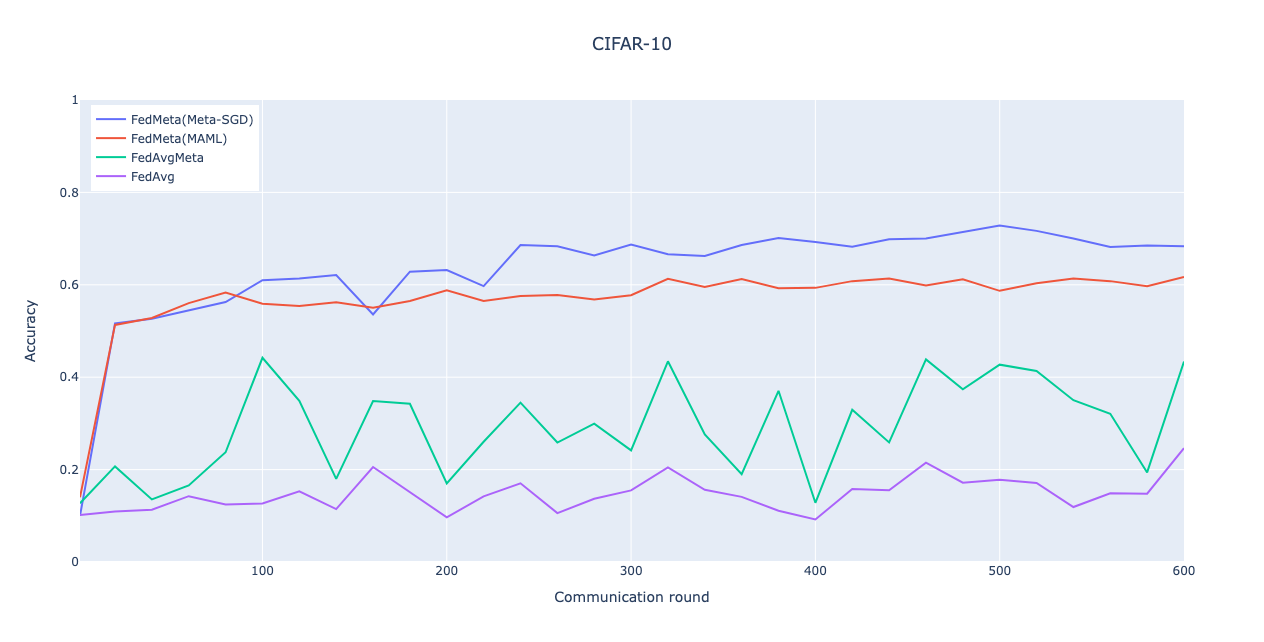
\includegraphics[width=\linewidth]{./images/cifar_meta_new.png}
            \caption{CIFAR-10, new clients}
            \label{fig:cifar_meta_new}
        \end{subfigure}%
        \begin{subfigure}{.5\textwidth}
            \centering
            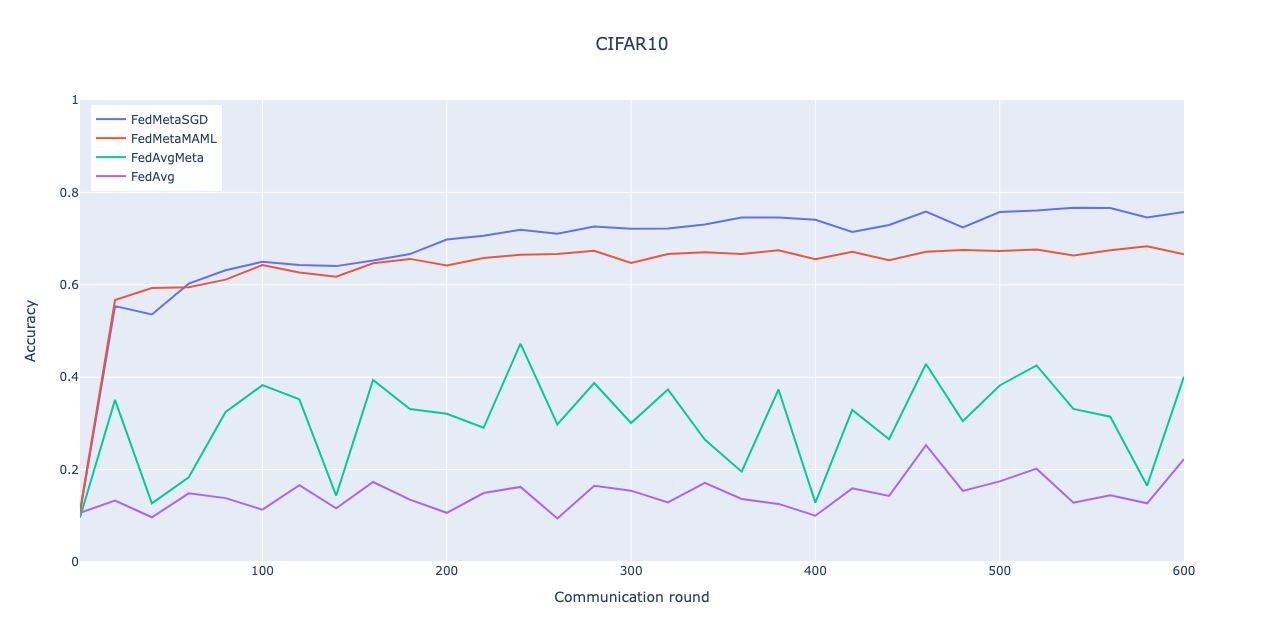
\includegraphics[width=\linewidth]{./images/cifar_meta_old.png}
            \caption{CIFAR-10, local clients}
            \label{fig:cifar_meta_old}
        \end{subfigure}
        % \caption{A figure with two subfigures}
        % \label{fig:test}
    \end{subfigure}

    \begin{subfigure}{\textwidth}
        \centering
        \begin{subfigure}{.5\textwidth}
            \centering
            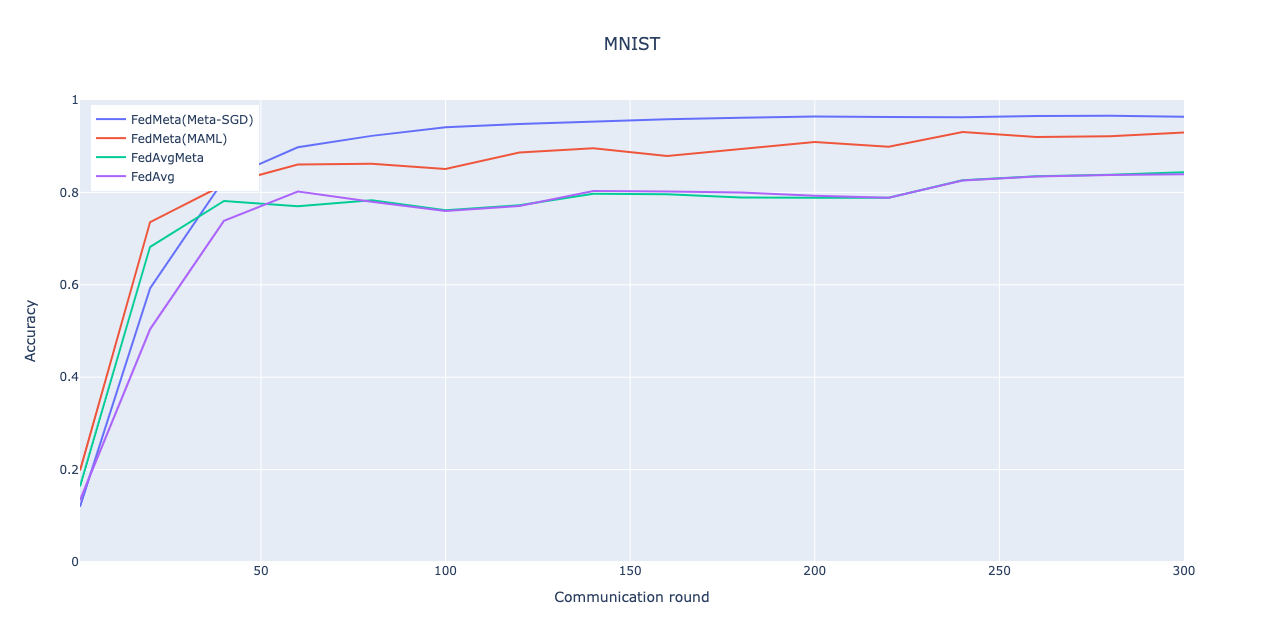
\includegraphics[width=\linewidth]{./images/mnist_meta_new.png}
            \caption{MNIST, new clients}
            \label{fig:mnist_meta_new}
        \end{subfigure}%
        \begin{subfigure}{.5\textwidth}
            \centering
            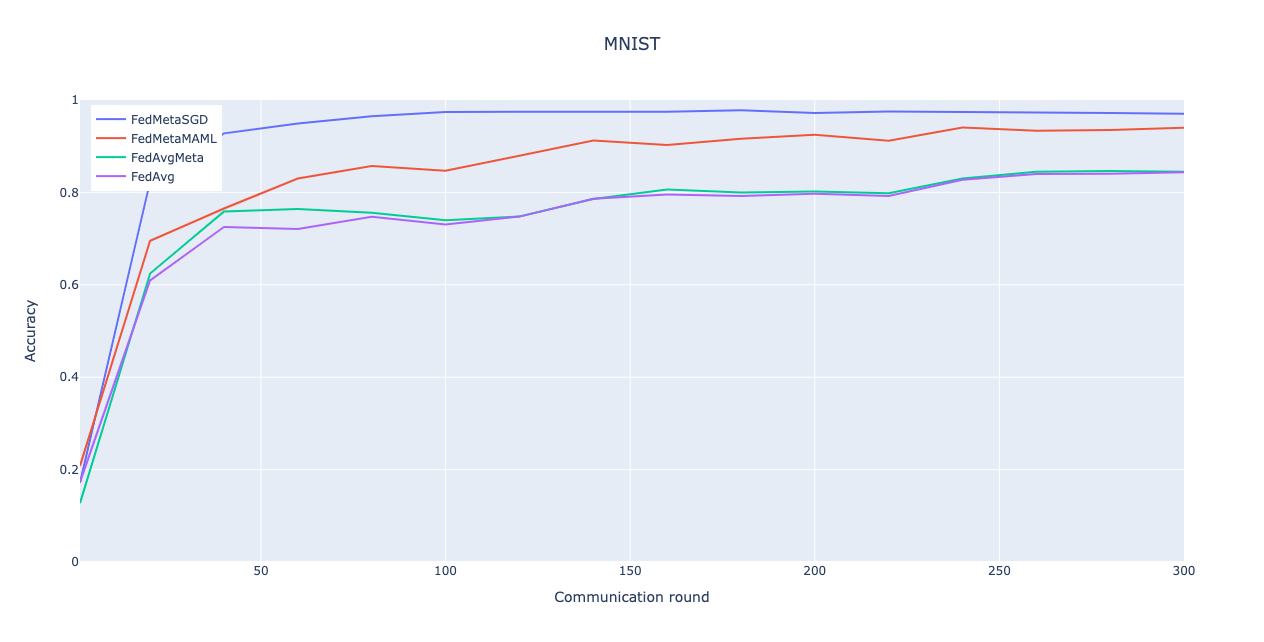
\includegraphics[width=\linewidth]{./images/mnist_meta_old.png}
            \caption{MNIST, local clients}
            \label{fig:mnist_meta_old}
        \end{subfigure}
        % \caption{A figure with two subfigures}
        % \label{fig:test}
    \end{subfigure}
    \caption{Kết quả chạy thuật toán FedAvg và các thuật toán FedMeta trên các tập dữ liệu và máy khách kiểm thử tương ứng}
    \label{fig:fedmeta_acc}
\end{sidewaysfigure}

\section{$FedMeta-Per$ trên dữ liệu Non-IID}

Với hai kỳ vọng vừa trình bày về khả năng thích ứng nhanh trên dữ liệu mới và khả năng cá nhân hóa mô hình học cho từng người dùng, khóa luận thử nghiệm thuật toán đề xuất trên hai tập dữ liệu CIFAR-10, MNIST và đạt được kết quả như bảng \ref{tab:fedmetaper_acc}. Theo đó, các thuật toán \codeword{FedMeta-Per} luôn cho kết quả cao nhất và cao hơn các thuật toán \codeword{FedPer} và \codeword{FedPerMeta} từ 2 đến 6 lần trên cả hai tập dữ liệu CIFAR-10 và MNIST.

\begin{table}
    \centering
    \caption{Bảng độ chính xác (\%) của thuật toán FedPer và các thuật toán FedMeta-Per tính trên điểm dữ liệu (dữ liệu Non-IID)}
    % \refstepcounter{table}
    \label{tab:fedmetaper_acc}
    \resizebox{\linewidth}{!}{%
    \begin{tabular}{l|cc|cc} 
    \toprule
                      & \multicolumn{2}{c|}{CIFAR-10}   & \multicolumn{2}{c}{MNIST}        \\ 
    \cline{2-5}
                      & local client   & new client     & local client   & new client      \\ 
    \hline
    FedPer            & 15.73          & 12.54          & 64.01          & 58.68           \\
    FedPerMeta        & 18.13          & 25.60          & 52.71          & 63.29           \\
    FedMeta-Per(MAML)     & 85.73          & 66.19          & \textbf{99.35}          & 93.21           \\
    FedMeta-Per(Meta-SGD) & \textbf{86.20} & \textbf{72.99} & 99.00 & \textbf{96.63}  \\
    \bottomrule
    \end{tabular}
    }
\end{table}

Xét về khả năng thích ứng nhanh trên tập dữ liệu mới, \codeword{FedMeta-Per} cho kết quả tốt hơn hẳn so với \codeword{FedPerMeta} khi cùng thực hiện một bước huấn luyện trên tập dữ liệu support (chỉ chiếm 20\% dữ liệu) của máy khách trong lúc kiểm thử, nhưng đã có thể nắm bắt được các đặc tính dữ liệu trong máy khách đó và cho kết quả dự đoán phân lớp với độ chính xác rất cao. Từ hình \ref{fig:fedmetaper_acc}, có thể quan sát thấy việc hội tụ của các thuật toán này cũng xảy ra nhanh hơn rất nhiều với hai thuật toán còn lại. Kết quả này tương đồng với kết quả thí nghiệm của các thuật toán \codeword{FedMeta}. Từ những ý phân tích vừa nêu, có thể kết luận rằng, \textbf{các thuật toán} \codeword{FedMeta-Per} \textbf{đã thừa hưởng thành công khả năng thích ứng nhanh trên tập dữ liệu mới của các thuật toán ML như đã kỳ vọng trước đó}.

\begin{table}
    \centering
    \caption{Bảng độ chính xác (\%) của thuật toán FedPer và các thuật toán FedMeta-Per tính trên máy khách (dữ liệu Non-IID)}
    \label{tab:fedmetaper_client_acc}
    \resizebox{\linewidth}{!}{%
    \begin{tabular}{l|cc|cc} 
    \toprule
                          & \multicolumn{2}{c|}{CIFAR-10}              & \multicolumn{2}{c}{MNIST}                  \\ 
    \cline{2-5}
                          & local client        & new client           & local client        & new client           \\ 
    \hline
    FedPer                & 15.41±20.90         & 13.91±20.40          & 63.67±20.04         & 55.06±26.09           \\
    FedPerMeta            & 17.46±23.15         & 20.99±22.61          & 54.94±23.14         & 59.43±27.31          \\
    FedMeta-Per(MAML)     & 85.58±7.40          & 61.81±21.63          & \textbf{99.33±0.89} & 94.06±7.73           \\
    FedMeta-Per(Meta-SGD) & \textbf{86.10±6.42} & \textbf{67.21±16.57} & 98.69±1.41          & \textbf{95.33±6.59}  \\
    \bottomrule
    \end{tabular}
    }
\end{table}

Khả năng cá nhân hóa mô hình cho từng người dùng được đánh giá dựa vào độ chính xác trong tương quan với máy khách, trình bày trong bảng \ref{tab:fedmetaper_client_acc}. Bảy trong số tám các trường hợp các thuật toán \codeword{FedMeta-Per} có độ lệch chuẩn nhỏ hơn thuật toán \codeword{FedPer} (trừ trường hợp kiểm định thuật toán \codeword{FedMeta-Per(MAML)} trên người dùng mới của tập CIFAR-10). Điều này chứng tỏ rằng khả năng cá nhân hóa của thuật toán đề xuất tốt hơn so với thuật toán \codeword{FedPer} và \codeword{FedPerMeta}.

Mặt khác, khóa luận so sánh các thuật toán \codeword{FedMeta} với các thuật toán \codeword{FedMeta-Per} và tổng hợp kết quả trong hai bảng \ref{tab:compare} và \ref{tab:compare_again}. Theo đó, độ chính xác của \codeword{FedMeta-Per} luôn cao hơn \codeword{FedMeta} từ 1\% đến 19\% khi so sánh trên cùng thuật toán huấn luyện cục bộ. Tính cá nhân hóa của \codeword{FedMeta-Per} cũng cao hơn đáng kể so với \codeword{FedMeta} khi thuật toán đề xuất, trong đa số các trường hợp, đã làm giảm độ lệch chuẩn của độ chính xác xuống từ 2 đến 10 lần xét trên cùng thuật toán huấn luyện cục bộ.

\begin{table}
    \centering
    \caption{Bảng so sánh độ chính xác (\%) giữa FedMeta và FedMeta-Per tính trên điểm dữ liệu (dữ liệu Non-IID)}
    \label{tab:compare}
    \resizebox{\linewidth}{!}{%
    \begin{tabular}{l|cc|cc} 
    \toprule
                          & \multicolumn{2}{c|}{CIFAR-10}   & \multicolumn{2}{c}{MNIST}        \\ 
    \cline{2-5}
                          & local client   & new client     & local client   & new client      \\ 
    \hline
    FedMeta(MAML)         & 66.58          & 64.86          & 93.09          & 92.55           \\
    FedMeta(Meta-SGD)     & 75.75          & 70.02          & 97.36          & 95.89           \\
    FedMeta-Per(MAML)     & 85.73          & 66.19          & \textbf{99.35} & 93.21           \\
    FedMeta-Per(Meta-SGD) & \textbf{86.20} & \textbf{72.99} & 99.00          & \textbf{96.63}  \\
    \bottomrule
    \end{tabular}
    }
\end{table}

\begin{table}
    \centering
    \caption{Bảng so sánh độ chính xác (\%) giữa FedMeta và FedMeta-Per tính trên máy khách (dữ liệu Non-IID)}
    \label{tab:compare_again}
    \resizebox{\linewidth}{!}{%
    \begin{tabular}{l|cc|cc} 
    \toprule
                          & \multicolumn{2}{c|}{CIFAR-10}              & \multicolumn{2}{c}{MNIST}                  \\ 
    \cline{2-5}
                          & local client        & new client           & local client        & new client           \\ 
    \hline
    FedMeta(MAML)         & 66.31±13.72         & 61.34±19.99          & 92.63±5.04          & 92.79±5.29           \\
    FedMeta(Meta-SGD)     & 76.01±11.98         & \textbf{67.98±15.28}          & 92.21±10.19         & 90.45±11.18          \\
    FedMeta-Per(MAML)     & 85.58±7.40          & 61.81±21.63          & \textbf{99.33±0.89} & 94.06±7.73           \\
    FedMeta-Per(Meta-SGD) & \textbf{86.10±6.42} & 67.21±16.57          & 98.69±1.41          & \textbf{95.33±6.59}  \\
    \bottomrule
    \end{tabular}
    }
\end{table}

\begin{sidewaysfigure}
    \centering
    \begin{subfigure}{\textwidth}
        \centering
        \begin{subfigure}{.5\textwidth}
            \centering
            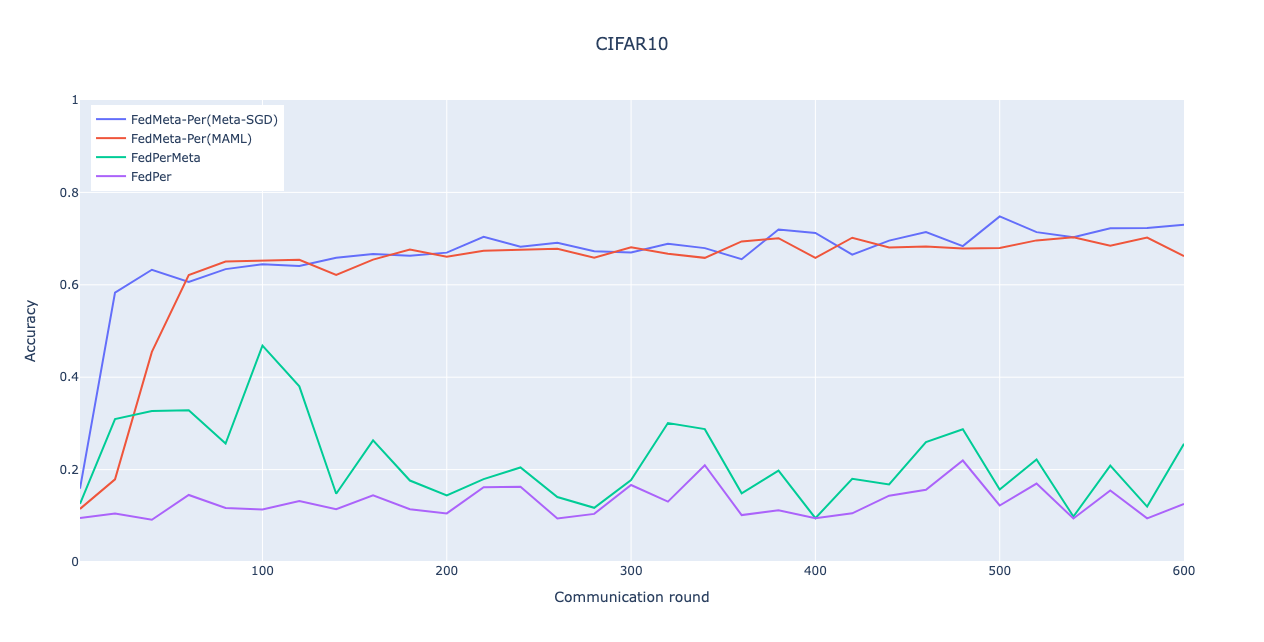
\includegraphics[width=\linewidth]{./images/cifar_per_new.png}
            \caption{CIFAR-10, new clients}
            \label{fig:cifar_per_new}
        \end{subfigure}%
        \begin{subfigure}{.5\textwidth}
            \centering
            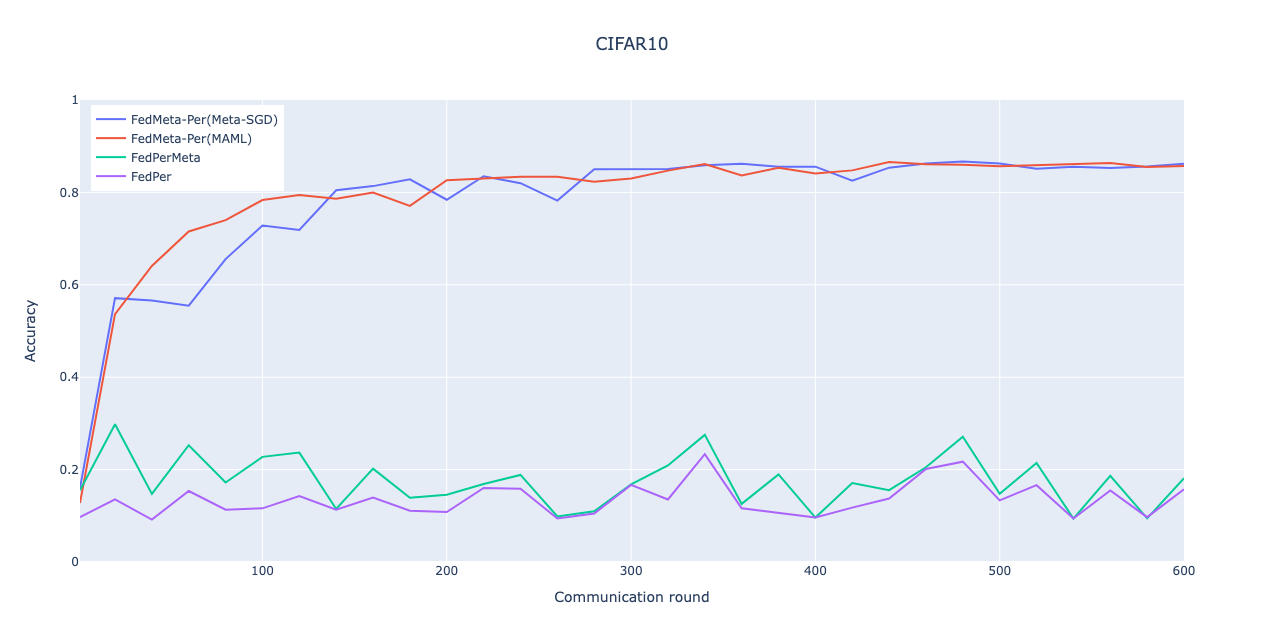
\includegraphics[width=\linewidth]{./images/cifar_per_old.png}
            \caption{CIFAR-10, local clients}
            \label{fig:cifar_per_old}
        \end{subfigure}
        % \caption{A figure with two subfigures}
        % \label{fig:test}
    \end{subfigure}

    \begin{subfigure}{\textwidth}
        \centering
        \begin{subfigure}{.5\textwidth}
            \centering
            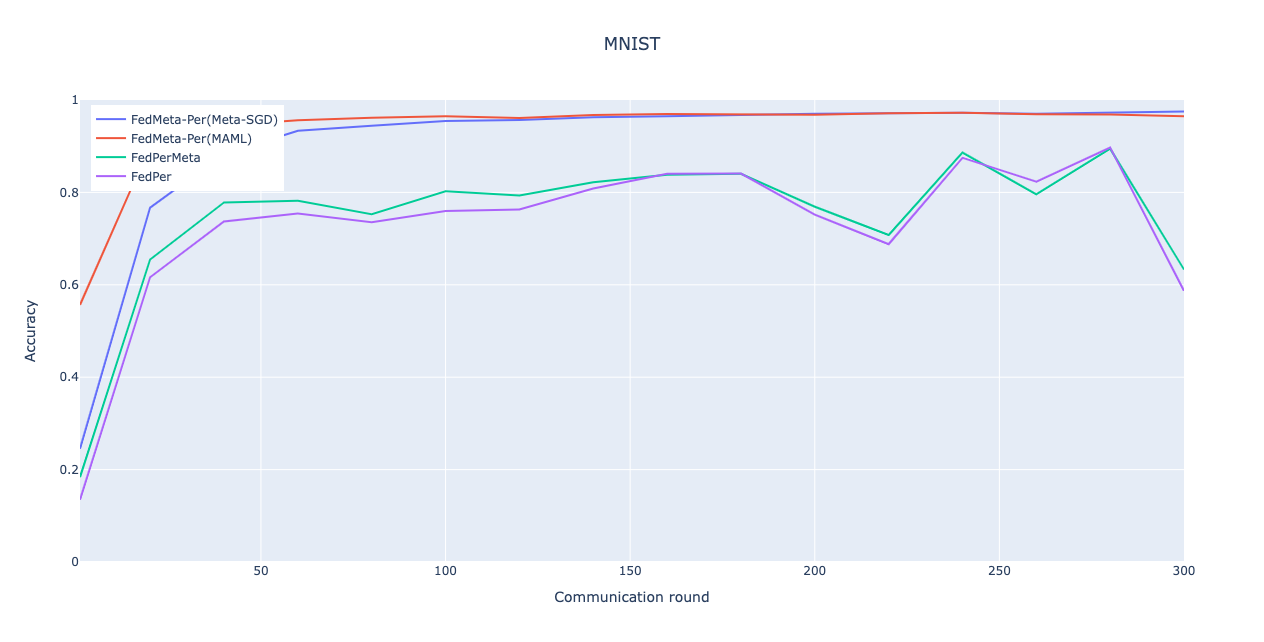
\includegraphics[width=\linewidth]{./images/mnist_per_new.png}
            \caption{MNIST, new clients}
            \label{fig:mnist_per_new}
        \end{subfigure}%
        \begin{subfigure}{.5\textwidth}
            \centering
            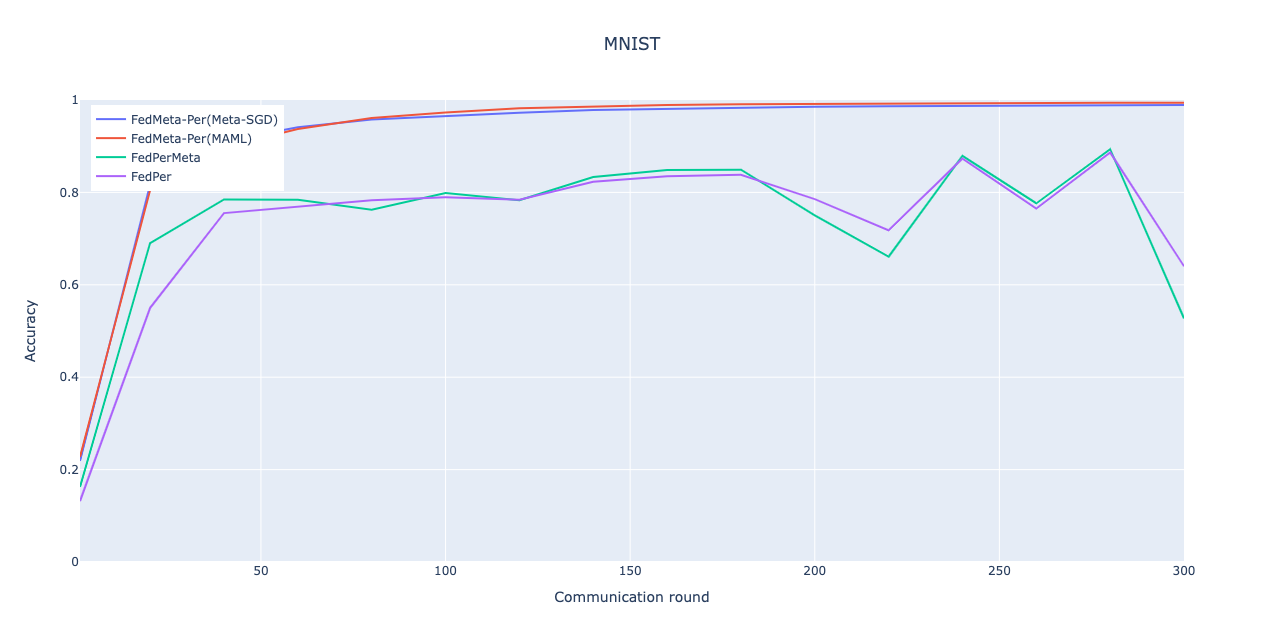
\includegraphics[width=\linewidth]{./images/mnist_per_old.png}
            \caption{MNIST, local clients}
            \label{fig:mnist_per_old}
        \end{subfigure}
        % \caption{A figure with two subfigures}
        % \label{fig:test}
    \end{subfigure}
    \caption{Kết quả chạy thuật toán FedPer và các thuật toán FedMeta-Per trên các tập dữ liệu và máy khách kiểm thử tương ứng}
    \label{fig:fedmetaper_acc}
\end{sidewaysfigure}
